\chapter{Introduction}
%New possiblities
Computing power and efficiency in modern processing chips and thus on \ac{sc} has risen exceptionally over the last decade. This opened the gate to machine learning and large deep neural networks. Twenty years ago it was infeasible or almost impossible to set up neural networks without an super-computer, while today reasonably big nets can be run on the average personal computer or even smart-phone \cite{efficient-nn}. Thus today, \ac{ai} with neural networks of any kind is considered to be used on \ac{sc} where computational power is still sparse due to long lead times and high requirements in the space industry. \newline
%Autonomy
Automatization can be found everywhere nowadays in this world. And especially space mission have a high demand on autonomous and intelligent decision making. The reasons are high delays due to long communication distances (e.g. deep space missions) or sparse ground contact, as well as the need for fast and independent decisions (e.g. Mars rover \cite{mars-ai} or rocket control \cite{rocket-control}). \newline 
%Thesis Goal (Uncertainty prediction and datamining)
So far \ac{ai} with neural networks has only been used in special cases in the space sector and is still under great research with various aspects which we will examine in the following sections. The focus in this thesis lies mainly within using neural networks to predict future values in time-series and tell the uncertainty of said prediction. The secondary focus is to gather the data and get it in the right format for the neural network, this process falls under topics data processing or data mining as well as feature engineering.

%Section Introduction
The introduction will first start off with \ac{ai} and machine learning, and sort various terms and definitions. With this theoretical side, the practical side will follow and examine corner stones in the latest research showing the state of the art w.r.t. autonomy, \ac{ai} and data mining. Following that, the case study (the Rosetta Mission \cite{rosetta-url}) will be presented, which is of special interest as it is a deep space mission with data over 10 years and with the occurrence of a anomalous friction values in two of the four reaction wheels.

\section{Artificial Intelligence}
%Introduce and distinguish A.I. / M.L. / D.L
Artificial intelligence describes a very broad area and includes simple algorithms as well as the realm of machine and deep learning. In figure \ref{f:ai_hierarchy} an inclusion diagram is given to show the three areas of interest here. The outer edge forms the general artificial intelligence. Within lies the machine learning, which is already the starting point of our journey. \ac{ml} describes a process of automated pattern learning or classification without explicit programming. This already concerns the build of neural networks leading to the area of deep learning. The building blocks of a neural network are - as the name suggests - artificial neurons; in the following they will be called \textit{nodes}. They have two fundamental properties, their inputs and their activation function at their output. Multiple nodes stacked in a vector fashion form a layer, as depicted in figure \ref{f:nn_example}. The outputs of theses nodes can be directed to the next layer, where they are summed up on the input of the next node within the layer. Mathematically this can be described as a function consisting of matrix multiplications:

\begin{equation}
f(\mathbf{x}; \mathbf{W}, \mathbf{c}, \mathbf{w}, b) = \mathbf{w}^T\cdot \left(\mathbf{W}\cdot \mathbf{x} + \mathbf{c} \right) + b
\end{equation}

This describes the exception of a network with one layer and one output, whereas $\mathbf{x}$ is the input vector, $\mathbf{W}$ the weight matrix with a bias vector $\mathbf{c}$ connecting the input with the hidden layer. $\mathbf{w}$ is a weight matrix for the hidden layer output. Additionally a constant bias $b$ is added to the function. The nodes in the hidden layer can have a activation function $\varphi_k(\hat{x_n})$ applied element-wise. The activation function defines how a node responds to its inputs, which is usually in a non-linear fashion.

%A.I. / M.L. / D.L.
\begin{figure}[htb]
\centering
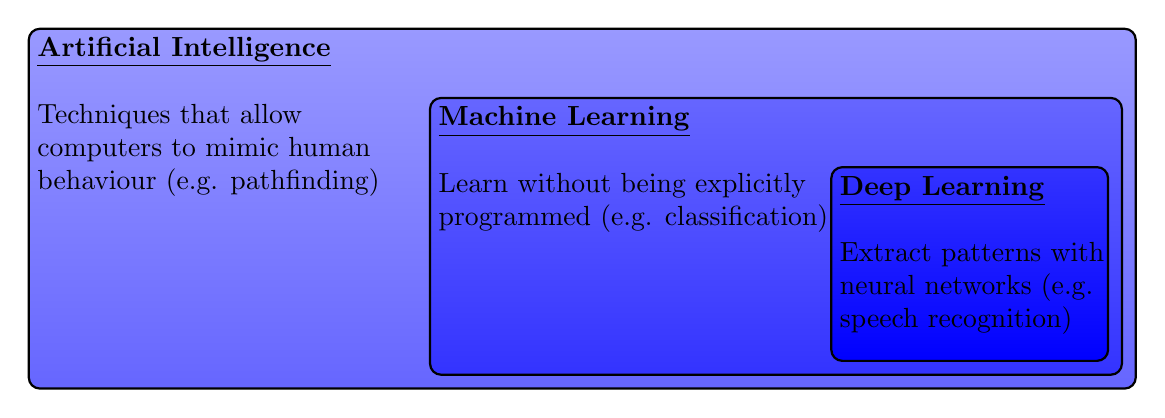
\begin{tikzpicture}[
    block/.style={
      rectangle,
      draw=black,
      thick,
      align=center,
      rounded corners,
      minimum height=5em,
	  minimum width=15em
    },
]

\node[block, top color=blue!40, bottom color=blue!60, minimum width=40em, minimum height=13em] (AI) at (0,0) {};
\node[below right, align=left] at (AI.north west) {\underline{\textbf{Artificial Intelligence}} 
\\ \\ Techniques that allow \\ computers to mimic human \\ behaviour (e.g. pathfinding)};

\node[block, top color=blue!60, bottom color=blue!80, minimum width=25em, minimum height=10em] (ML) at (7em,-1em) {};
\node[below right, align=left] at (ML.north west) {\underline{\textbf{Machine Learning}}
\\ \\ Learn without being explicitly \\ programmed (e.g. classification)};

\node[block, top color=blue!80, bottom color=blue!100, minimum width=10em, minimum height=7em] (DL) at (14em,-2em) {};
\node[below right, align=left] at (DL.north west) {\underline{\textbf{Deep Learning}}
\\ \\ Extract patterns with \\ neural networks (e.g. \\ speech recognition)};

\end{tikzpicture}

\caption{Hierarchy of Artificial Intelligence, Machine Learning and Deep Learning.}
\label{f:ai_hierarchy}
\end{figure}

%Neural Network
\begin{figure}[htb]
\centering
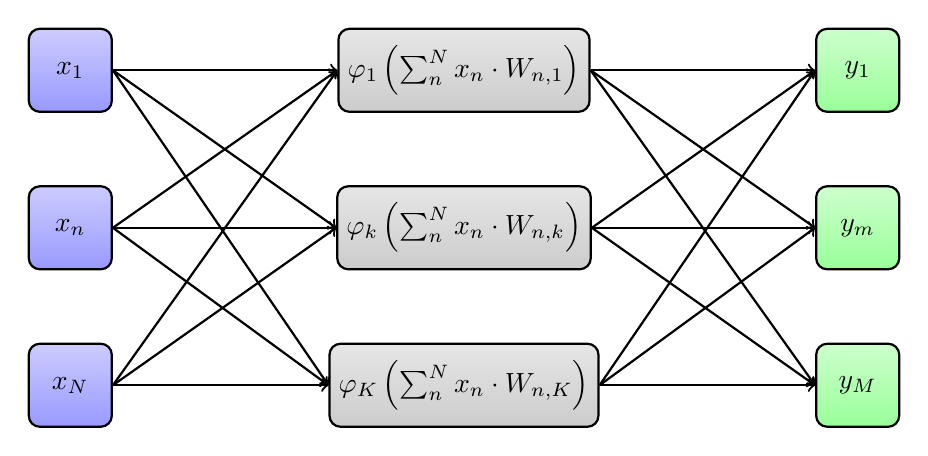
\begin{tikzpicture}[
	input/.style={
		rectangle,
		draw=black,
		thick,
		align=center,
		rounded corners,
		top color=blue!20,
		bottom color=blue!40,
		minimum height=3em,
		minimum width=3em
	},
	neuron/.style={
		rectangle,
		draw=black,
		thick,
		align=center,
		rounded corners,
		top color=gray!20,
		bottom color=gray!40,
		minimum height=3em,
		minimum width=3em
	},
	output/.style={
		rectangle,
		draw=black,
		thick,
		align=center,
		rounded corners,
		top color=green!20,
		bottom color=green!40,
		minimum height=3em,
		minimum width=3em
	},
]

\node[input] (in1) at (-5, 2) {$x_1$};
\node[input] (in2) at (-5, 0) {$x_n$};
\node[input] (in3) at (-5, -2) {$x_N$};

\node[neuron] (nin1) at (0, 2) {$\varphi_1 \left(\sum_n^N x_n\cdot W_{n,1}\right)$};
\node[neuron] (nin2) at (0, 0) {$\varphi_k \left(\sum_n^N x_n\cdot W_{n,k}\right)$};
\node[neuron] (nin3) at (0, -2) {$\varphi_K \left(\sum_n^N x_n\cdot W_{n,K}\right)$};

\draw[thick,->] (in1.east) -- (nin1.west);
\draw[thick,->] (in1.east) -- (nin2.west);
\draw[thick,->] (in1.east) -- (nin3.west);

\draw[thick,->] (in2.east) -- (nin1.west);
\draw[thick,->] (in2.east) -- (nin2.west);
\draw[thick,->] (in2.east) -- (nin3.west);

\draw[thick,->] (in3.east) -- (nin1.west);
\draw[thick,->] (in3.east) -- (nin2.west);
\draw[thick,->] (in3.east) -- (nin3.west);

\node[output] (out1) at (5, 2) {$y_1$};
\node[output] (out2) at (5, 0) {$y_m$};
\node[output] (out3) at (5, -2) {$y_M$};

\draw[thick,->] (nin1.east) -- (out1.west);
\draw[thick,->] (nin1.east) -- (out2.west);
\draw[thick,->] (nin1.east) -- (out3.west);

\draw[thick,->] (nin2.east) -- (out1.west);
\draw[thick,->] (nin2.east) -- (out2.west);
\draw[thick,->] (nin2.east) -- (out3.west);

\draw[thick,->] (nin3.east) -- (out1.west);
\draw[thick,->] (nin3.east) -- (out2.west);
\draw[thick,->] (nin3.east) -- (out3.west);

\end{tikzpicture}

\caption{\ac{fnn} with input $\mathbf{x}$ and length $N$, a neuron layer with length $K$ connecting the input vector via a weight matrix $\mathbf{W}$. The output vector $\mathbf{y}$ with length $N$ is formed with the activation function $\varphi_k(\hat{x_k})$ and another weight matrix $\mathbf{w}$.}
\label{f:nn_example}
\end{figure}

This kind of network is called a \ac{fnn}. It can be \textit{shallow} if it only has one layer and \textit{deep} if it has multiple (hidden) layers.

The other two network types of concern here are the \acp{cnn} \cite[p. 321ff]{deep-learning} and the \acp{rnn} \cite[p. 363ff]{deep-learning} which will be introduced once we start to build a neural network model in chapter \ref{c:nn-blocks}.

\section{State of the Art}
%Introduce ai and datamining
As the use of \ac{ml} in space is rather new, we will concentrate mostly on the last twenty years of research. The data mining in contrast dates back many decades more and will be the fundamental base for the neural network input.

%Introduce autonomy, datamining and uncertainty
The question of autonomy in space has been around since the first day of space travel as the environment is hostile towards humans and the effort for manual intervention quite high. \newline
Below a definition of autonomy will be roughly outlined and referred to further sources. The first step to autonomous decision-making is the pre-processing or data mining of all gathered data. Here we introduce techniques to gain first information about the data itself and make it ready to be fed into a neural network. The neural network is then used to generated future predictions of the processed input data. Our focus of this prediction is the uncertainty, which is grossly underestimated in its importance. 

\subsection{AI for Autonomy in Space}
Autonomy is a word that can mean various levels of self-organizing and acting in an mostly new or unknown environment. This starts with simple boundary checks tackling single instances of subsystems up to complex decisions affecting the whole system functionality. To put this into numbers and general definitions, four levels of autonomy in ascending order are given by the \ac{ecss} \cite{ecss-autonomy}:

\begin{enumerate}
\item[E1:] Mission execution under ground control with limited on-board capability for safety issues
\item[E2:] Execution of pre-planned, ground-defined, mission operations on-board
\item[E3:] Execution of adaptive mission operations on-board
\item[E4:] Execution of goal-oriented mission operations on-board
\end{enumerate}

The ultimate goal would be of course to reach the autonomy level E4. Here, in this thesis our \ac{ai} is a \ac{nn} and concerned with predictions and uncertainty. The prediction itself can already be used to find and mitigate possible safety issues and anomalies in housekeeping data. Secondly it can be used to guide a spacecraft or rover by estimating the (un-)certainty of possible future actions. Therefore our \ac{nn} can be put in a category somewhere between E1 and E2. \newline
To go further and reach higher levels, one would need an ensemble of \acp{nn} covering every subsystems. On the highest level these \acp{nn} would need to be bound to an pre-defined expert system. The reason for an expert system lies in the very nature of \acp{nn} and the area of machine learning itself as these networks have to be trained for their specific task. But as space mission and their goals are usually unique, there is no real possibility to train an \ac{ai} for a space mission.

In real missions, autonomy and especially \ac{ai} have been used in a more sparse and specific context. One example is ATHMOS at the \ac{dlr}, where a neural network was used to predict future housekeeping values $\num{4.5}$ hours into the future with high accuracy \cite{athmos} \cite{athmos-sub}.

\subsection{Data Mining}
Data mining is an interdisciplinary approach over many scientific fields. It is situated somewhere between data processing, informatics and machine learning, and therefore mostly concerned with acquiring data, finding raw statistical features and patterns, and making predictions. For us it is merely a necessary step towards the following data analysis and seldom a part of the analysis itself. Therefore we are strictly using the pre-processing parts to fit the data to our needs and to ensure the data is neither ill conditioned nor corrupted. The basis for the data mining forms the book by Ian Davidson and Xinguqan Zhu \cite{data-mining}.

For the use of any further computation, the data has to be checked for validity and a constant sampling rate. Here statistical features like minimum, maximum, mean and variance can be calculated to get a first insight. Also the data has to be checked for gaps and obvious anomalies. \newline
One essential tool in the field of data mining is the \ac{ssa}, where a data series is analysed by its frequency components. Here we will take a look at the X-11 method, which is one realisation of the \ac{ssa}.

\subsubsection{X-11}
The X-11 method originates from the US Bureau of the Census and was developed to represent economic models for seasonal and trend analysis \cite[p. 1f]{x11-book}. The season therefore obviously spans here over the course of one year on earth to account for the typical cycle of weekends, holidays, festive days and climate seasons. As a result, it can be used to estimate future trends (month or quarter) to make political and economic decisions. 

The X-11 method has already shown on satellite data, that a decomposition and analysis is possible and useful \cite{tm-mining}. Hence it will be used in this work as a rough baseline to see how far a statistical method can reach and how much further the machine learning techniques can go.

Fortunately, the X-11 method is already implemented in Python\footnote{Script language \url{python.org}} and can be used out of the box in a non-parametric way with an adjustable window size.

\subsection{Uncertainty Prediction}
For the neural networks that are about to be built and analysed, not only a future prediction, but also a uncertainty prediction has to be made. Uncertainty can occur in various places, in the data, the model and the prediction. To build a neural network with a known uncertainty or the uncertainty as an additional output, some extra steps have to be taken. The usual output of a neural network is just a simple value or vector telling the learned result or prediction. In case of a classification problem it tells the most likely class the input belongs to. For a regression it might be a prediction value or polynomial fit-function. \newline
To understand the additional uncertainty we will look at an example. If one wants to classify cats and dogs via pictures, the \ac{nn} will have two classes/outputs belonging to the respective classes. The output values are probabilities $P(x=x_i)$ for the associated class appearing in the input $x_i$. The sum of probabilities over all known classes is:

\begin{equation}
\sum_i P(x=x_i)=1
\end{equation}

If one would now feed in a picture of a horse, the \ac{nn} would still predict how likely it saw a cat or a dog, where neither is true. Therefore a secondary output would be needed on how certain the \ac{nn} is about its prediction. In the case of a horse picture, the certainty for the two classes cat or dog would be very low.

One important research in this area has been done in the thesis from Yarin Gal \cite{yarin-thesis} and the derived paper \cite{yarin-dropout} where he first showed the theory behind the hidden uncertainty in neural networks and secondly how to directly extract uncertainty parameters. \newline
Starting in 2019 Googles Tensorflow \cite{tf-web} has caught up to this area and developed a framework for using probability distributions in \acp{nn} called \enquote{tensorflow probability}. In chapter \ref{c:prediction} we will dive into this framework, examine how it works and use it for our predictions.

\section{Example Case - Rosetta Mission}
To test and show our neural networks as well as their predictions and the uncertainty, a real world example case is needed. For that the Rosetta Mission \cite{rosetta-url} from \ac{esa} was chosen. The mission was launched in 2004 and sent towards the comet Tschurjumow-Gerassimenko, which it did reach in 2014. On its way it made several turns in the solar system with various swing-bys to gain speed and also intermediate science missions on the asteroid Steins (2007) and Lutetia (2011). After Lutetia, Rosetta was set into a hibernation state to save energy until it reached its final destination.

In our case, we are not interested in the scientific missions and findings, but in the housekeeping data of the \ac{sc}. For Rosetta this data is freely available on \cite{rosetta-data}, together with the manuals on the instruments functionality and how to interpret their measurements \cite{rosetta-manual}. \newline
Our special interests in the housekeeping data are for one the reaction wheels and second the solar arrays. The reaction wheels are of interest as they failed and showed anomalies during the mission \cite{rosetta-maintenance}. As a countermeasure the failing wheels were also re-lubricated. With our \ac{nn} we want to see, if we are able to predict this anomalous behaviour. \newline
As second part we want to analyse the degradation of the solar arrays as data like this fits very well in the area of regression analysis and prediction.

A quick overview on the mission chronology to better understand the context of the housekeeping data is given in the next section.

\subsection{Chronology}
The Rosetta Mission started in 2004 and ended in 2016 with the impact on the comet Tschurjumow-Gerassimenko. In 2011 the \ac{sc} entered a hibernation phase where it was set inactive during the cruise to the final destination. As the reaction wheels had already failed before entering the hibernation, only the timeframe from 2004 to 2011 is considered for our later analysis. Therefore also the following event table \ref{t:rosetta_trajectory} only includes this timeframe.

The mission made several swing-bys on Earth and Mars before reaching its first target comet Steins. This means, that during that time (till the encounter of Steins), the \ac{sc} had an elliptically varying distance to the sun. As result, the solar arrays might perform differently with respect to the distance as well as the reaction wheels with different temperature equilibriums. After the asteroid encounter, the reaction wheel B already showed degradation and was lubricated twice after a swing by on earth in 2009. And in 2010 the reaction wheel B was turned off before the encounter with Lutetia. Just a few months later reaction wheel C showed an increased friction in August 2010 and was subsequently lubricated to restore performance \cite{rosetta-maintenance}.

All these events have to be taken into account and will be referred to when the data is analysed either statistically or via machine learning.

\begin{table}[htb]
\centering
\caption{Rosetta Trajectory and Events}
\begin{tabular}{b{0.2\textwidth}b{0.2\textwidth}b{0.5\textwidth}}
\toprule
Date 		& $\Delta t$[d] 						& Description \\  \midrule
2004-03-02	& $\SI{0}{\second}$				& Spacecraft launch \\
2005-03-04	& $\SI{31.7e6}{\second}$				& Swing by at Earth \\
2007-02-25	& $\SI{94.2e6}{\second}$				& Swing by at Mars \\
2007-11-13	& $\SI{116.7e6}{\second}$				& Swing by at Earth \\
2008-09-05	& $\SI{142.4e6}{\second}$				& Encounter with Steins \\
2008-09		& $\approx\SI{143.2e6}{\second}$		& RWA B increased friction \\
2009-11-13	& $\SI{179.9e6}{\second}$				& Swing by at Earth \\
2009-11		& $\approx\SI{180.1e6}{\second}$		& RWA B lubrication \\
2010-01		& $\approx\SI{185.4e6}{\second}$		& RWA B lubrication \\
2010-07		& $\approx\SI{199.8e6}{\second}$		& RWA B turned off \\
2010-07-10	& $\SI{200.5e6}{\second}$				& Encounter with Lutetia \\
2010-08		& $\approx\SI{202.4e6}{\second}$		& RWA C increased friction \\
2010			& $\approx\SI{207.7e6}{\second}$		& RWA C subsequent lubrication \\
2011-06-08	&  $\SI{229.3e6}{\second}$			& Hibernation Start \\
\bottomrule
\end{tabular}
\label{t:rosetta_trajectory}
\end{table}